%%%%%%%%%%%%%%%%%%%%%%%%%%%%%%%%%%%%%%%%%%%%%%%
%%%     Declarations (skip to Begin Document, line 88, for parts you fill in)
%%%%%%%%%%%%%%%%%%%%%%%%%%%%%%%%%%%%%%%%%%%%%%%

\documentclass[10pt]{article}

\usepackage{geometry}  % Lots of layout options.  See http://en.wikibooks.org/wiki/LaTeX/Page_Layout
\geometry{letterpaper}  % ... or a4paper or a5paper or ... 
\usepackage{fullpage}  % somewhat standardized smaller margins (around an inch)
\usepackage{setspace}  % control line spacing in latex documents
\usepackage[parfill]{parskip}  % Activate to begin paragraphs with an empty line rather than an indent

\usepackage{amsmath,amssymb}  % latex math
\usepackage{empheq} % http://www.ctan.org/pkg/empheq
\usepackage{bm,upgreek}  % allows you to write bold greek letters (upper & lower case)

% for typsetting algorithm pseudocode see http://en.wikibooks.org/wiki/LaTeX/Algorithms_and_Pseudocode
\usepackage{algorithmic,algorithm}  

\usepackage{graphicx}  % inclusion of graphics; see: http://en.wikibooks.org/wiki/LaTeX/Importing_Graphics
% allow easy inclusion of .tif, .png graphics

\usepackage{verbatim}
\DeclareGraphicsRule{.tif}{png}{.png}{`convert #1 `dirname #1`/`basename #1 .tif`.png}


% \usepackage{subfigure}  % allows subfigures in figure
\usepackage{caption}
\usepackage{subcaption}

\usepackage{xspace}
\newcommand{\latex}{\LaTeX\xspace}

\usepackage{color}  % http://en.wikibooks.org/wiki/LaTeX/Colors

\long\def\todo#1{{\color{red}{\bf TODO: #1}}}

\long\def\ans#1{{\color{blue}{\em #1}}}
\long\def\ansnem#1{{\color{blue}#1}}
\long\def\boldred#1{{\color{red}{\bf #1}}}
\long\def\boldred#1{\textcolor{red}{\bf #1}}
\long\def\boldblue#1{\textcolor{blue}{\bf #1}}

% Useful package for syntax highlighting of specific code (such as python) -- see below
\usepackage{listings}  % http://en.wikibooks.org/wiki/LaTeX/Packages/Listings
\usepackage{textcomp}

%%% The following lines set up using the listings package
\renewcommand{\lstlistlistingname}{Code Listings}
\renewcommand{\lstlistingname}{Code Listing}

%%% Specific for python listings
\definecolor{gray}{gray}{0.5}
\definecolor{green}{rgb}{0,0.5,0}

\lstnewenvironment{python}[1][]{
\lstset{
language=python,
basicstyle=\footnotesize,  % could also use this -- a little larger \ttfamily\small\setstretch{1},
stringstyle=\color{red},
showstringspaces=false,
alsoletter={1234567890},
otherkeywords={\ , \}, \{},
keywordstyle=\color{blue},
emph={access,and,break,class,continue,def,del,elif ,else,%
except,exec,finally,for,from,global,if,import,in,i s,%
lambda,not,or,pass,print,raise,return,try,while},
emphstyle=\color{black}\bfseries,
emph={[2]True, False, None, self},
emphstyle=[2]\color{green},
emph={[3]from, import, as},
emphstyle=[3]\color{blue},
upquote=true,
morecomment=[s]{"""}{"""},
commentstyle=\color{gray}\slshape,
emph={[4]1, 2, 3, 4, 5, 6, 7, 8, 9, 0},
emphstyle=[4]\color{blue},
literate=*{:}{{\textcolor{blue}:}}{1}%
{=}{{\textcolor{blue}=}}{1}%
{-}{{\textcolor{blue}-}}{1}%
{+}{{\textcolor{blue}+}}{1}%
{*}{{\textcolor{blue}*}}{1}%
{!}{{\textcolor{blue}!}}{1}%
{(}{{\textcolor{blue}(}}{1}%
{)}{{\textcolor{blue})}}{1}%
{[}{{\textcolor{blue}[}}{1}%
{]}{{\textcolor{blue}]}}{1}%
{<}{{\textcolor{blue}<}}{1}%
{>}{{\textcolor{blue}>}}{1},%
%framexleftmargin=1mm, framextopmargin=1mm, frame=shadowbox, rulesepcolor=\color{blue},#1
framexleftmargin=1mm, framextopmargin=1mm, frame=single,#1
}}{}
%%% End python code listing definitions

\DeclareMathOperator{\diag}{diag}
\DeclareMathOperator{\cov}{cov}

%%%%%%%%%%%%%%%%%%%%%%%%%%%%%%%%%%%%%%%%%%%%%%%
%%%     Begin Document
%%%%%%%%%%%%%%%%%%%%%%%%%%%%%%%%%%%%%%%%%%%%%%%

\begin{document}

\begin{center}
    {\Large {\bf ISTA 421/521 -- Homework 4}} \\
    \boldred{Due: Monday, October 29, 5pm} \\
    20 pts total for Undergrads, 25 pts total for Grads\\
    
\end{center}

\begin{flushright}
Ken Youens-Clark

Graduate
\end{flushright}

\vspace{1cm}

Note: I worked with Kai Blumberg and Matt Miller.

%%%%%%%%%%%%%%%%
%%%     Problems
%%%%%%%%%%%%%%%%

\begin{itemize}

%%%     Problem 1
\item[1.]  [5 points; \boldred{Required only for Graduates}]
Adapted from {\bf Exercise 3.12} of FCMA p.135:

When performing a Bayesian analysis of the Olympics data, we assumed that $\sigma^2$ was known.  If instead we assume that $\mathbf{w}$ is known and an inverse Gamma prior is placed on $\sigma^2$,
\begin{eqnarray*}
p(\sigma^2 | \alpha, \beta) = \frac{\beta^{\alpha}}{\Gamma(\alpha)} (\sigma^2)^{-\alpha-1} \exp \left\{-\frac{\beta}{\sigma^2} \right\},
\end{eqnarray*}
then the posterior over $\sigma^2$ will also be inverse Gamma.  Derive the parameters for the posterior belief in the variance.  

%Also, explain why this is a better prior than a Gaussian density.

{\bf Solution.}

The posterior will be a Gaussian over $\mathbf{w}$ times the given prior:

\begin{eqnarray*}
\begin{aligned}
p(\mathbf{w}|\mu, \sigma^2) p(\sigma^2 | \alpha, \beta) &= 
\frac{1}{(2 \pi)^{N/2} | \mathbf{\sigma}^2 \mathbf{I}|^{1/2}} 
\exp 
\left\{ 
-\frac{1}{2} 
(\mathbf{X}\mathbf{w} - \mathbf{t})^\top 
(\mathbf{\sigma}^2 \mathbf{I})^{-1} 
(\mathbf{X}\mathbf{w}- \mathbf{t}) 
\right\}
\\
&\times
\frac{\beta^{\alpha}}{\Gamma(\alpha)} (\sigma^2)^{-\alpha-1} 
\exp \left\{-\frac{\beta}{\sigma^2} \right\}
\\
&=
\left(
\frac{1}{(2 \pi)^{N/2} | \mathbf{\sigma}^2 \mathbf{I}|^{1/2}} 
\times
\frac{\beta^{\alpha}}{\Gamma(\alpha)} (\sigma^2)^{-\alpha-1}
\right)
\exp \left\{
-\frac{1}{2} (\mathbf{X}\mathbf{w}- \mathbf{t})^\top 
(\mathbf{\sigma}^2 \mathbf{I})^{-1} (\mathbf{X}\mathbf{w} - \mathbf{t}) 
-
\frac{\beta}{\sigma^2} 
\right\}
\\
&=
\left(
\frac{1}{(2 \pi)^{N/2}} 
\times \frac{1}{| \mathbf{\sigma}^2 \mathbf{I}|^{1/2}} 
\times
\frac{\beta^{\alpha}}{\Gamma(\alpha)}
\times
(\sigma^2)^{-\alpha-1}
\right)
\exp \left\{
-\frac{1}{2\sigma^2} (\mathbf{X}\mathbf{w} - \mathbf{t})^\top (\mathbf{X}\mathbf{w} - \mathbf{t})
- \frac{\beta}{\sigma^2}
\right\}
\\
&=
\left(
\frac{1}{(2 \pi)^{N/2}} 
\times \frac{1}{| \mathbf{\sigma}^2 \mathbf{I}|^{1/2}} 
\times
\frac{\beta^{\alpha}}{\Gamma(\alpha)}
\times
(\sigma^2)^{-\alpha-1}
\right)
\exp \left\{
-\frac{1}{2\sigma^2} ((\mathbf{X}\mathbf{w})^\top - \mathbf{t}^\top) (\mathbf{X}\mathbf{w} - \mathbf{t})
- \frac{\beta}{\sigma^2}
\right\}
\\
&=
\left(
\frac{1}{(2 \pi)^{N/2}} 
\times \frac{1}{| \mathbf{\sigma}^2 \mathbf{I}|^{1/2}} 
\times
\frac{\beta^{\alpha}}{\Gamma(\alpha)}
\times
(\sigma^2)^{-\alpha-1}
\right)
\exp \left\{
\frac{
-\frac{1}{2}((\mathbf{X}\mathbf{w})^\top \mathbf{X}\mathbf{w} 
- 2 \mathbf{w}^\top \mathbf{X}^\top \mathbf{t}
+ \mathbf{t}^\top \mathbf{t}) - \beta}
{\sigma^2}
\right\}
\\
&=
\left(
\frac{1}{|\mathbf{\sigma}^2 \mathbf{I}|^{1/2}} 
\times
(\sigma^2)^{-\alpha-1}
\right)
\exp \left\{
\frac{
- \frac{1}{2}((\mathbf{X}\mathbf{w})^\top \mathbf{X}\mathbf{w}) 
+ \mathbf{w}^\top \mathbf{X}^\top \mathbf{t}
- \frac{1}{2} \mathbf{t}^\top \mathbf{t} - \beta}
{\sigma^2}
\right\}
\\
&=
\left(
\frac{(\sigma^2)^{-\alpha-1}}{(\sigma^2)^{D/2}}
\right)
\exp \left\{
\frac{
- \frac{1}{2}((\mathbf{X}\mathbf{w})^\top \mathbf{X}\mathbf{w}) 
+ \mathbf{w}^\top \mathbf{X}^\top \mathbf{t}
- \frac{1}{2} \mathbf{t}^\top \mathbf{t} - \beta}
{\sigma^2}
\right\}
\\
&=
\left(
(\sigma^2)^{-\alpha-1} (\sigma^2)^{-D/2}
\right)
\exp \left\{
\frac{
- \frac{1}{2}((\mathbf{X}\mathbf{w})^\top \mathbf{X}\mathbf{w}) 
+ \mathbf{w}^\top \mathbf{X}^\top \mathbf{t}
- \frac{1}{2} \mathbf{t}^\top \mathbf{t} - \beta}
{\sigma^2}
\right\}
\\
&=
\left(
(\sigma^2)^{(-\alpha - D/2 - 1)}
\right)
\exp \left\{
\frac{
- \frac{1}{2}((\mathbf{X}\mathbf{w})^\top \mathbf{X}\mathbf{w}) 
+ \mathbf{w}^\top \mathbf{X}^\top \mathbf{t}
- \frac{1}{2} \mathbf{t}^\top \mathbf{t} - \beta}
{\sigma^2}
\right\}
\\
\hat{\alpha} &= \alpha + D/2
\\
\hat{\beta} &=
- \frac{1}{2}((\mathbf{X}\mathbf{w})^\top \mathbf{X}\mathbf{w}) 
+ \mathbf{w}^\top \mathbf{X}^\top \mathbf{t}
- \frac{1}{2} \mathbf{t}^\top \mathbf{t} - \beta
\end{aligned}
\end{eqnarray*}

%%%     Problem 2
\item[2.]  [6 points]
Adapted from {\bf Exercise 4.2} of FCMA p.163:

In Chapter 3, we computed the posterior density over $r$, the probability of a coin giving heads, using a beta prior and a binomial likelihood.  Recalling that the beta prior, with parameters $\alpha$ and $\beta$, is given by
\begin{eqnarray*}
p(r | \alpha, \beta) = \frac{\Gamma(\alpha + \beta)}{\Gamma(\alpha) \Gamma(\beta)} r^{\alpha - 1} (1 - r)^{\beta - 1}
\end{eqnarray*}
and the binomial likelihood, assuming $y$ heads in $N$ throws, is given by
\begin{eqnarray*}
p(y | r, N) = {N \choose y} r^{y} (1 - r)^{N-y} ~,
\end{eqnarray*}
{\bf compute the Laplace approximation to the posterior}.  (Note, you should be able to obtain a closed-form solution for the MAP value, $\hat{r}$, by getting the log posterior, differentiating (with respect to $r$), equating to zero and solving for $r$.)

{\bf Solution.}
\begin{eqnarray*}
\begin{aligned}
f &= p(r|\alpha, \beta) p(y|r,N) 
\\
&\propto r^{\alpha + y_N - 1}(1 -r)^{\beta + N - y_N - 1}
\\
&\propto r^{\delta - 1}(1 -r)^{\gamma - 1}
\\
&\text{where $\delta = y_N + \alpha$ and $\gamma = N - y_N + \beta$}
\\
\log(f) &= \log(r)(\delta - 1) + \log(1 - r)(\gamma - 1)
\\
\frac{\partial \log(f)}{\partial r} 
&= \frac{\delta - 1}{r} - \frac{\gamma - 1}{1 - r} = 0
\\
\frac{\delta - 1}{r} &= \frac{\gamma - 1}{1 - r}
\\
(\delta - 1)(1-r) &= r(\gamma - 1)
\\
\delta - r\delta - 1 + r &= r\gamma - r
\\
2r - r\delta - r\gamma &= 1 - \delta 
\\
r(2 - \delta - \gamma) &= 1 - \delta
\\
\hat{r} &= \frac{1 - \delta}{2 - \delta - \gamma} 
\\
\hat{r} &= \frac{1 - (y_N + \alpha)}{ 2 - (y_N + \alpha) - (N - y_N + \beta)}
\\
\hat{r} &= \frac{1 - y_N - \alpha}{ 2 - y_N - \alpha - N + y_N - \beta}
\\
\hat{r} &= \frac{1 - y_N - \alpha}{ 2 - \alpha - N - \beta}
\\
\frac{\partial \log(f)}{\partial r} &= \frac{\delta - 1}{r} - \frac{\gamma - 1}{1 - r}
\\
&= r^{-1}(\delta - 1) - (1 - r)^{-1}(\gamma - 1)
\\
\frac{\partial^2 \log(f)}{\partial r} 
&= - r^{-2}(\delta - 1) - (1 - r)^{-2}(\gamma - 1)\\
&= - \frac{y_N + \alpha - 1}{r^2} - \frac{(N - y_N + \beta - 1)}{(1-r)^2}
\end{aligned}
\end{eqnarray*}

The Laplace approximation is $\mathcal{N}(\mu, \Sigma)$ where

\begin{eqnarray*}
\begin{aligned}
\mu &= \hat{r}
\\
\Sigma^{-1} &= - \left( \frac{\partial^2 \log(f)}{\partial r} \right) \Big|_{\hat{r}}
\end{aligned}
\end{eqnarray*}


%%%     Problem 3
\item[3.]  [4 points]
Adapted from {\bf Exercise 4.3} of FCMA p.163:

In the previous exercise you computed the Laplace approximation to the true beta posterior.  In this problem, plot both the true beta posterior and the Laplace approximation for the following three parameter settings:
\begin{enumerate}
\item $\alpha = 5$, $\beta = 5$, $N = 20$, and $y = 10$,
\item $\alpha = 3$, $\beta = 15$, $N = 10$, and $y = 3$,
\item $\alpha = 1$, $\beta = 30$, $N = 10$, and $y = 3$.
\end{enumerate}
Be sure to clearly indicate the values in your plot captions.  Include how the two distributions (the true beta posterior and the Laplace approximation) compare in each case.  Include the python script you use to generate these plots; the script should be named {\tt plot\_laplace\_approx.py}.  {\bf Suggestion}: for plotting the beta and Gaussian (Normal) distributions, you can use {\tt scipy.stats.beta} and {\tt scipy.stats.normal} to create the beta and Gaussian random variables, and use the {\tt pdf(x)} method for each to generate the curves.  Note that for {\tt scipy.stats.normal}, the mean is the location ({\tt loc}) parameter, and the sigma is the {\tt scale} parameter.  Also, {\tt scipy.stats.normal} expects the scale parameter to be the standard deviation (i.e., take the square root: {\tt math.sqrt(x)}) of the variance you'll compute for the Laplace approximation.


{\bf Solution.}

\begin{figure}[H]
\centering
  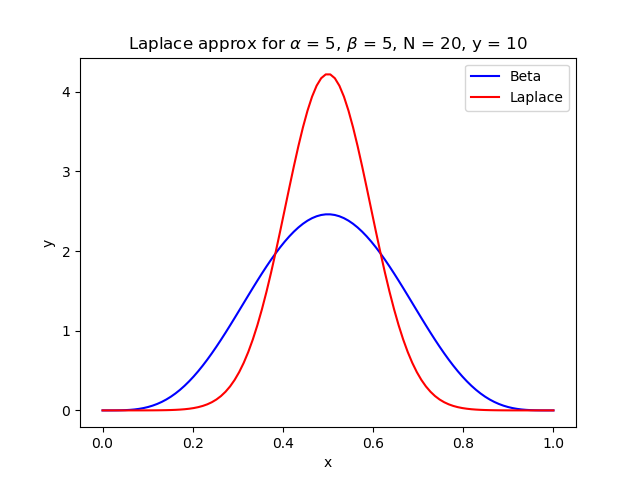
\includegraphics[width=\linewidth]{laplace1.png}
 \caption{Laplace approximation of Beta distibution for $\alpha = 5, \beta = 5, N = 20, y = 10$.}
\label{label}
\end{figure}

Here the Laplace approximation can easily match the mode but overshoots the intensity. Overall this is a lackluster fit. 

\begin{figure}[H]
\centering
  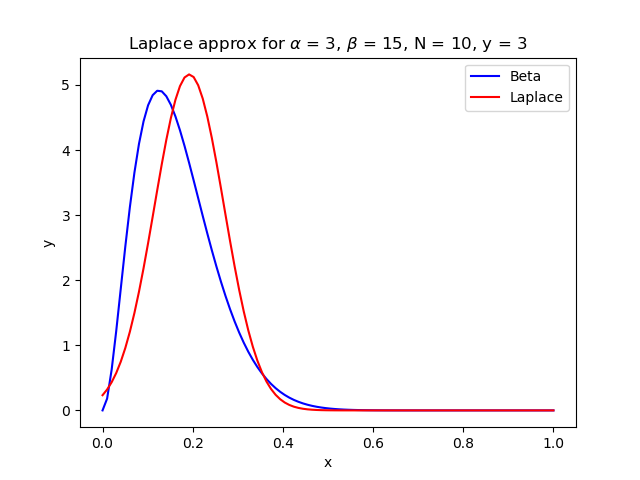
\includegraphics[width=\linewidth]{laplace2.png}
 \caption{Laplace approximation of Beta distibution for $\alpha = 3, \beta = 15, N = 10, y = 3$.}
\label{label}
\end{figure}

The approximation seems quite good in shape though it slightly misses the peak in both location and size.

\begin{figure}[H]
\centering
  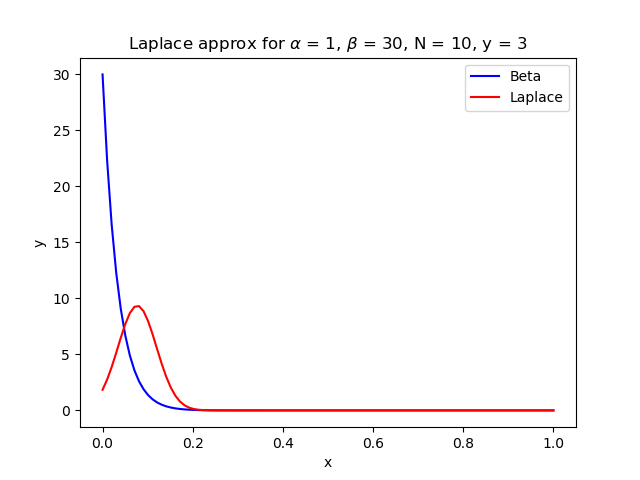
\includegraphics[width=\linewidth]{laplace3.png}
 \caption{Laplace approximation of Beta distibution for $\alpha = 1, \beta = 30, N = 10, y = 3$.}
\label{label}
\end{figure}

The approximation is not able to show the true Beta form's heavily skewed distribution to the left.

Following is my code to plot these:

\verbatiminput{plot_laplace_approx.py}

%%%     Problem 4
\item[4.]  [4 points]
Adapted from {\bf Exercise 4.4} of FCMA p.164:

Given the expression for the area of a circle, $A = \pi r^2$, and {\em using only uniformly distributed random variates}, devise a sampling approach for estimating $\pi$.  Describe your method in detail and provide your script to do the estimation -- this script should be called {\tt pi\_sample\_estimate.py}.  Report your estimate based on 1 million samples to 6 decimal places.  (NOTE: You do {\em not} need to use Metropolis-Hastings to compute this.)

{\bf Solution.} %$<$Solution goes here$>$

Here is the code I wrote:

\verbatiminput{pi_sample_estimate.py}

Here is the code with the default value of 1M samples:

\begin{verbatim}
$ ./pi_sample_estimate.py
pi ~ 3.138772
$ ./pi_sample_estimate.py
pi ~ 3.140552
$ ./pi_sample_estimate.py
pi ~ 3.141736
$ ./pi_sample_estimate.py
pi ~ 3.140920
\end{verbatim}

It's interesting to compare to fewer samples:

\begin{verbatim}
$ ./pi_sample_estimate.py -n 1000
pi ~ 3.156000
$ ./pi_sample_estimate.py -n 10000
pi ~ 3.146000
$ ./pi_sample_estimate.py -n 100000
pi ~ 3.135040
\end{verbatim}

%%%     Problem 5
\item[5.]  [6 points]
Adapted from {\bf Exercise 4.6} of FCMA p.164:

Assume that we observe $N$ vectors of attributes, $\mathbf{x}_1, ..., \mathbf{x}_N$, and associated integer counts $t_1, ..., t_N$.  A Poisson likelihood would be suitable:
\begin{eqnarray*}
p(t_n | \mathbf{x}_n, \mathbf{w}) = \frac{f(\mathbf{x}_n; \mathbf{w})^{t_n} \exp \{ -f(\mathbf{x}_n; \mathbf{w}) \}}{t_n!},
\end{eqnarray*}
where $f(\mathbf{x}_n;\mathbf{w}) = \mathbf{w}^\top\mathbf{x}_n$.
Assuming a zero-mean Gaussian prior on $\mathbf{w}$ with constant diagonal covariance of $\sigma^2$, derive the gradient and Hessian of the posterior.  Using these, express the parameter update rules for (a) gradient {\em ascent} (because we're maximizing) update (in class we looked at Widrow-Hoff, which is typically expressed for {\em descent}), and (b) Newton-Raphson.

The following facts will help in the derivation.  First, keep in mind that although $\mathbf{w}$ and $\mathbf{x}_n$ are vectors (of the same dimension), their dot product, $\mathbf{w}^\top\mathbf{x}_n$, is a {\em scalar} value.  This means you can take the partial derivative of $\log \mathbf{w}^\top\mathbf{x}_n$ with respect to $\mathbf{w}$.  Also, remember that the Hessian is a matrix representing the second partial derivatives of the gradient with respect to itself (see Comment 2.6 of p.73), and the second derivative will involve the {\em transpose} of the partial derivative with respect to $\mathbf{w}$.  So, e.g., as part of taking the second derivative, if you are taking the transpose derivative part of $\mathbf{w}^\top\mathbf{x}_n$, as follows:
\begin{eqnarray*}
\frac{\partial (\mathbf{w}^\top \mathbf{x}_n)}{\partial \mathbf{w}} = \mathbf{x}_n
~~~~\mathrm{and}~~~~
\frac{\partial (\mathbf{w}^\top \mathbf{x}_n)}{\partial \mathbf{w}^\top} = \mathbf{x}_n^\top
\end{eqnarray*}

{\bf Solution.} %$<$Solution goes here$>$

\begin{eqnarray*}
\begin{aligned}
\text{The Gaussian prior}
\\
p(\mathbf{w}|\mu, \sigma^2) &=
\frac{1}{(2 \pi)^{N/2} | \sigma^2 \mathbf{I}|^{1/2}} 
\exp 
\left\{ 
-\frac{1}{2} 
(\mathbf{w}\ - \mu)^\top 
(\sigma^2 \mathbf{I})^{-1} 
(\mathbf{w}\ - \mu)
\right\}
\\
\text{Since $\mu = 0$}
\\ 
&= \frac{1}{(2 \pi \sigma^2)^{D/2}} 
\exp 
\left\{ 
-\frac{1}{2\sigma^2} 
\mathbf{w}^\top \mathbf{w}
\right\}
\\
f = p(t_n | \mathbf{x}_n, \mathbf{w}) p(\mathbf{w}|\mu, \sigma^2)
&=\frac{(\mathbf{w}^\top\mathbf{x}_n)^{t_n} 
\exp \{ - \mathbf{w}^\top\mathbf{x}_n  \}}{t_n!} 
\times
\frac{1}{(2 \pi \sigma^2)^{D/2}} 
\exp 
\left\{ 
-\frac{1}{2\sigma^2} \mathbf{w}^\top \mathbf{w}
\right\}
\\
% log
\log(f) &= t_n \log(\mathbf{w}^\top \mathbf{x}_n) + (-\mathbf{w}^\top \mathbf{x}_n) - \log(t_n!)
+ \log(\frac{1}{(2 \pi \sigma^2)^{D/2}}) - \frac{1}{2\sigma^2} \mathbf{w}^\top \mathbf{w}
\\
% 1st derivative
\frac{\partial \log(f)}{\partial \mathbf{w}} 
&= t_n \mathbf{x}_n (\mathbf{w}^\top \mathbf{x}_n)^{-1} - \mathbf{x}_n - \frac{1}{\sigma^2}\mathbf{w}
\\
% 2nd derivatice
\frac{\partial^2 \log(f)}{\partial \mathbf{w} \partial \mathbf{w}^\top } &=
-( t_n \mathbf{x}_n^\top \mathbf{x}_n ( \mathbf{w}^\top \mathbf{x}_n)^{-2}) - \frac{1}{\sigma^2}
\end{aligned}
\end{eqnarray*}

(a)  Widrow-Hoff update:
\begin{eqnarray*}
\begin{aligned}
w_{n+1} &= w_n + \alpha \left(\frac{\partial \log(f)}{\partial \mathbf{w}}\right)
\\
&= w_n + \alpha \left(
t_n \mathbf{x}_n (\mathbf{w}^\top \mathbf{x}_n)^{-1} 
- \mathbf{x}_n - \frac{1}{\sigma^2}\mathbf{w}
\right)
\end{aligned}
\end{eqnarray*}

(b)  Newton-Raphson update:
\begin{eqnarray*}
\begin{aligned}
w_{n+1} &= w_n - 
\left(
\frac{\partial^2 \log(f)}{\partial \mathbf{w} \partial \mathbf{w}^\top }
\right)^{-1}
\frac{\partial \log(f)}{\partial \mathbf{w}}
\\
&= w_n - 
\left(
-( t_n \mathbf{x}_n^\top \mathbf{x}_n ( \mathbf{w}^\top \mathbf{x}_n)^{-2}) - \frac{1}{\sigma^2}
\right)^{-1}
\left(
t_n \mathbf{x}_n (\mathbf{w}^\top \mathbf{x}_n)^{-1} - \mathbf{x}_n - \frac{1}{\sigma^2}\mathbf{w}
\right)
\end{aligned}
\end{eqnarray*}

\end{itemize}

\end{document}
